\chapter{Design og implementering}

\section{Software Design}

\subsection{Devkit8000}

\subsubsection{Candydriver}
Candydriveren sørger for SPI-kommunikationen fra Devkit8000 til PSoC0. SPI-kommunikationen er implementeret med SPI bus nummer 1, SPI chip-select 0 og en hastighed på 1 MHz (et godt stykke under max på 20 MHz for en sikkerhedsskyld). Desuden starter clocken højt og data ændres på falling edge og aflæses på rising edge. Dermed bliver SPI Clock Mode 3. Derudover sendes der 8 bit pr transmission, hvilket passer med SPI-protokollen for projektet.\\
For at kunne anvende driveren, når SPI er tilsluttet, er der oprettet et hotplugmodul, som fortæller kernen, at der er et SPI device, som matcher driveren. Det kan SPI-forbindelsen ikke selv gøre, som usb fx kan. Selve driveren er i candygun.c opbygget som en char driver. For at holde forskellige funktionaliteter adskilt er alle funktioner, der har med SPI at gøre, implementeret i filen candygun-spi-c. Så når der fx skal requestes en SPI ressource i init-funktionen i candygun.c, så anvender driveren en funktion fra candygun-spi.c til det. I probe-funktionen sættes bits\textunderscore per\textunderscore word til 8, da vi sender otte bit som nævnt tidligere. I exit-funktionen anvender candygun.c igen en funktion fra candygun-spi.c - denne gang til at frigive SPI ressourcen. I write-metoden gives der data med fra brugeren. I dette tilfælde udgøres brugeren af Interface driveren og dataet er en 8 bit kommando fra SPI-protokollen. Dog er dataet fra brugeren i første omgang læst ind som en charstreng. I write-metoden bliver det så lavet om til en int.  For at overføre dataet på en sikker måde anvendes funktionen copy\textunderscore from\textunderscore user() til at overføre data fra brugeren. Write-funktionen fra candygun.c anvender derefter en write-funktion fra candygun-spi.c, hvor den sender brugerinputtet med. I den spi-relaterede write-funktion bliver bruger inputtet lagt i transfer bufferen og der NULL bliver lagt i receive bufferen, og med spi\textunderscore sync-funktionen bliver det sendt. \\ 
Ofte ville der en spi read-funktion først indeholde en write-del, som fortalte SPI-slaven, hvad der skulle læses over i bufferen. Det ville typisk efterfølges af et delay og så en read-del. Men i dette projekt skal der ofte afventes et brugerinput, som ikke kan styres af et fast delay, og der skal generelt sendes en aktiv kommando før der læses. Derfor er det besluttet at read-funktionen kun indeholder en read-del i transmissionen. Dermed skal write-funktionen altid aktivt anvendes inden der læses, da PSoC0 ellers ikke ved, hvad der skal gøres/lægges i bufferen.\\
Når funktionen har modtaget resultatet fra transmissionen returneres det til brugeren med funktionen copy\textunderscore to\textunderscore user(), som igen sørger for at overførslen af data foregår på en sikker måde.



\subsubsection{Interfacedriver}
Interface driveren er bindeled mellem brugergrænsefladen og candydriveren. Interface driveren er implementeret i c++ og opbygget med klasserelationen arv. Den indeholder tre funktioner til use case 2. De håndterer test af de forskellige kommunikationsforbindelser i systemet. Der er en basisklasse, ICandyGun, som er abstrakt, da alle metoder er virtuelle. Derudover er der to afledte klasser, SimulCandyGun og RealCandyGun. SimulCandyGun simulerer svaret på funktionerne ved brug af rand()-funktionen. Den sikrer at brugergrænsefladen kan testes uden at være forbundet til det resterende system. RealCandyGun klassen implementerer de rigtig funktioner med forbindelse til det restende system, og anvender de nødvendige funktioner til at skrive til og læse fra et kernemodul. På figur \ref{fig:IDriverKlasseDiagram} ses klassediagrammet for arvehierarkiet i Interface Driveren. 

\begin{figure}[H]
	\centering
	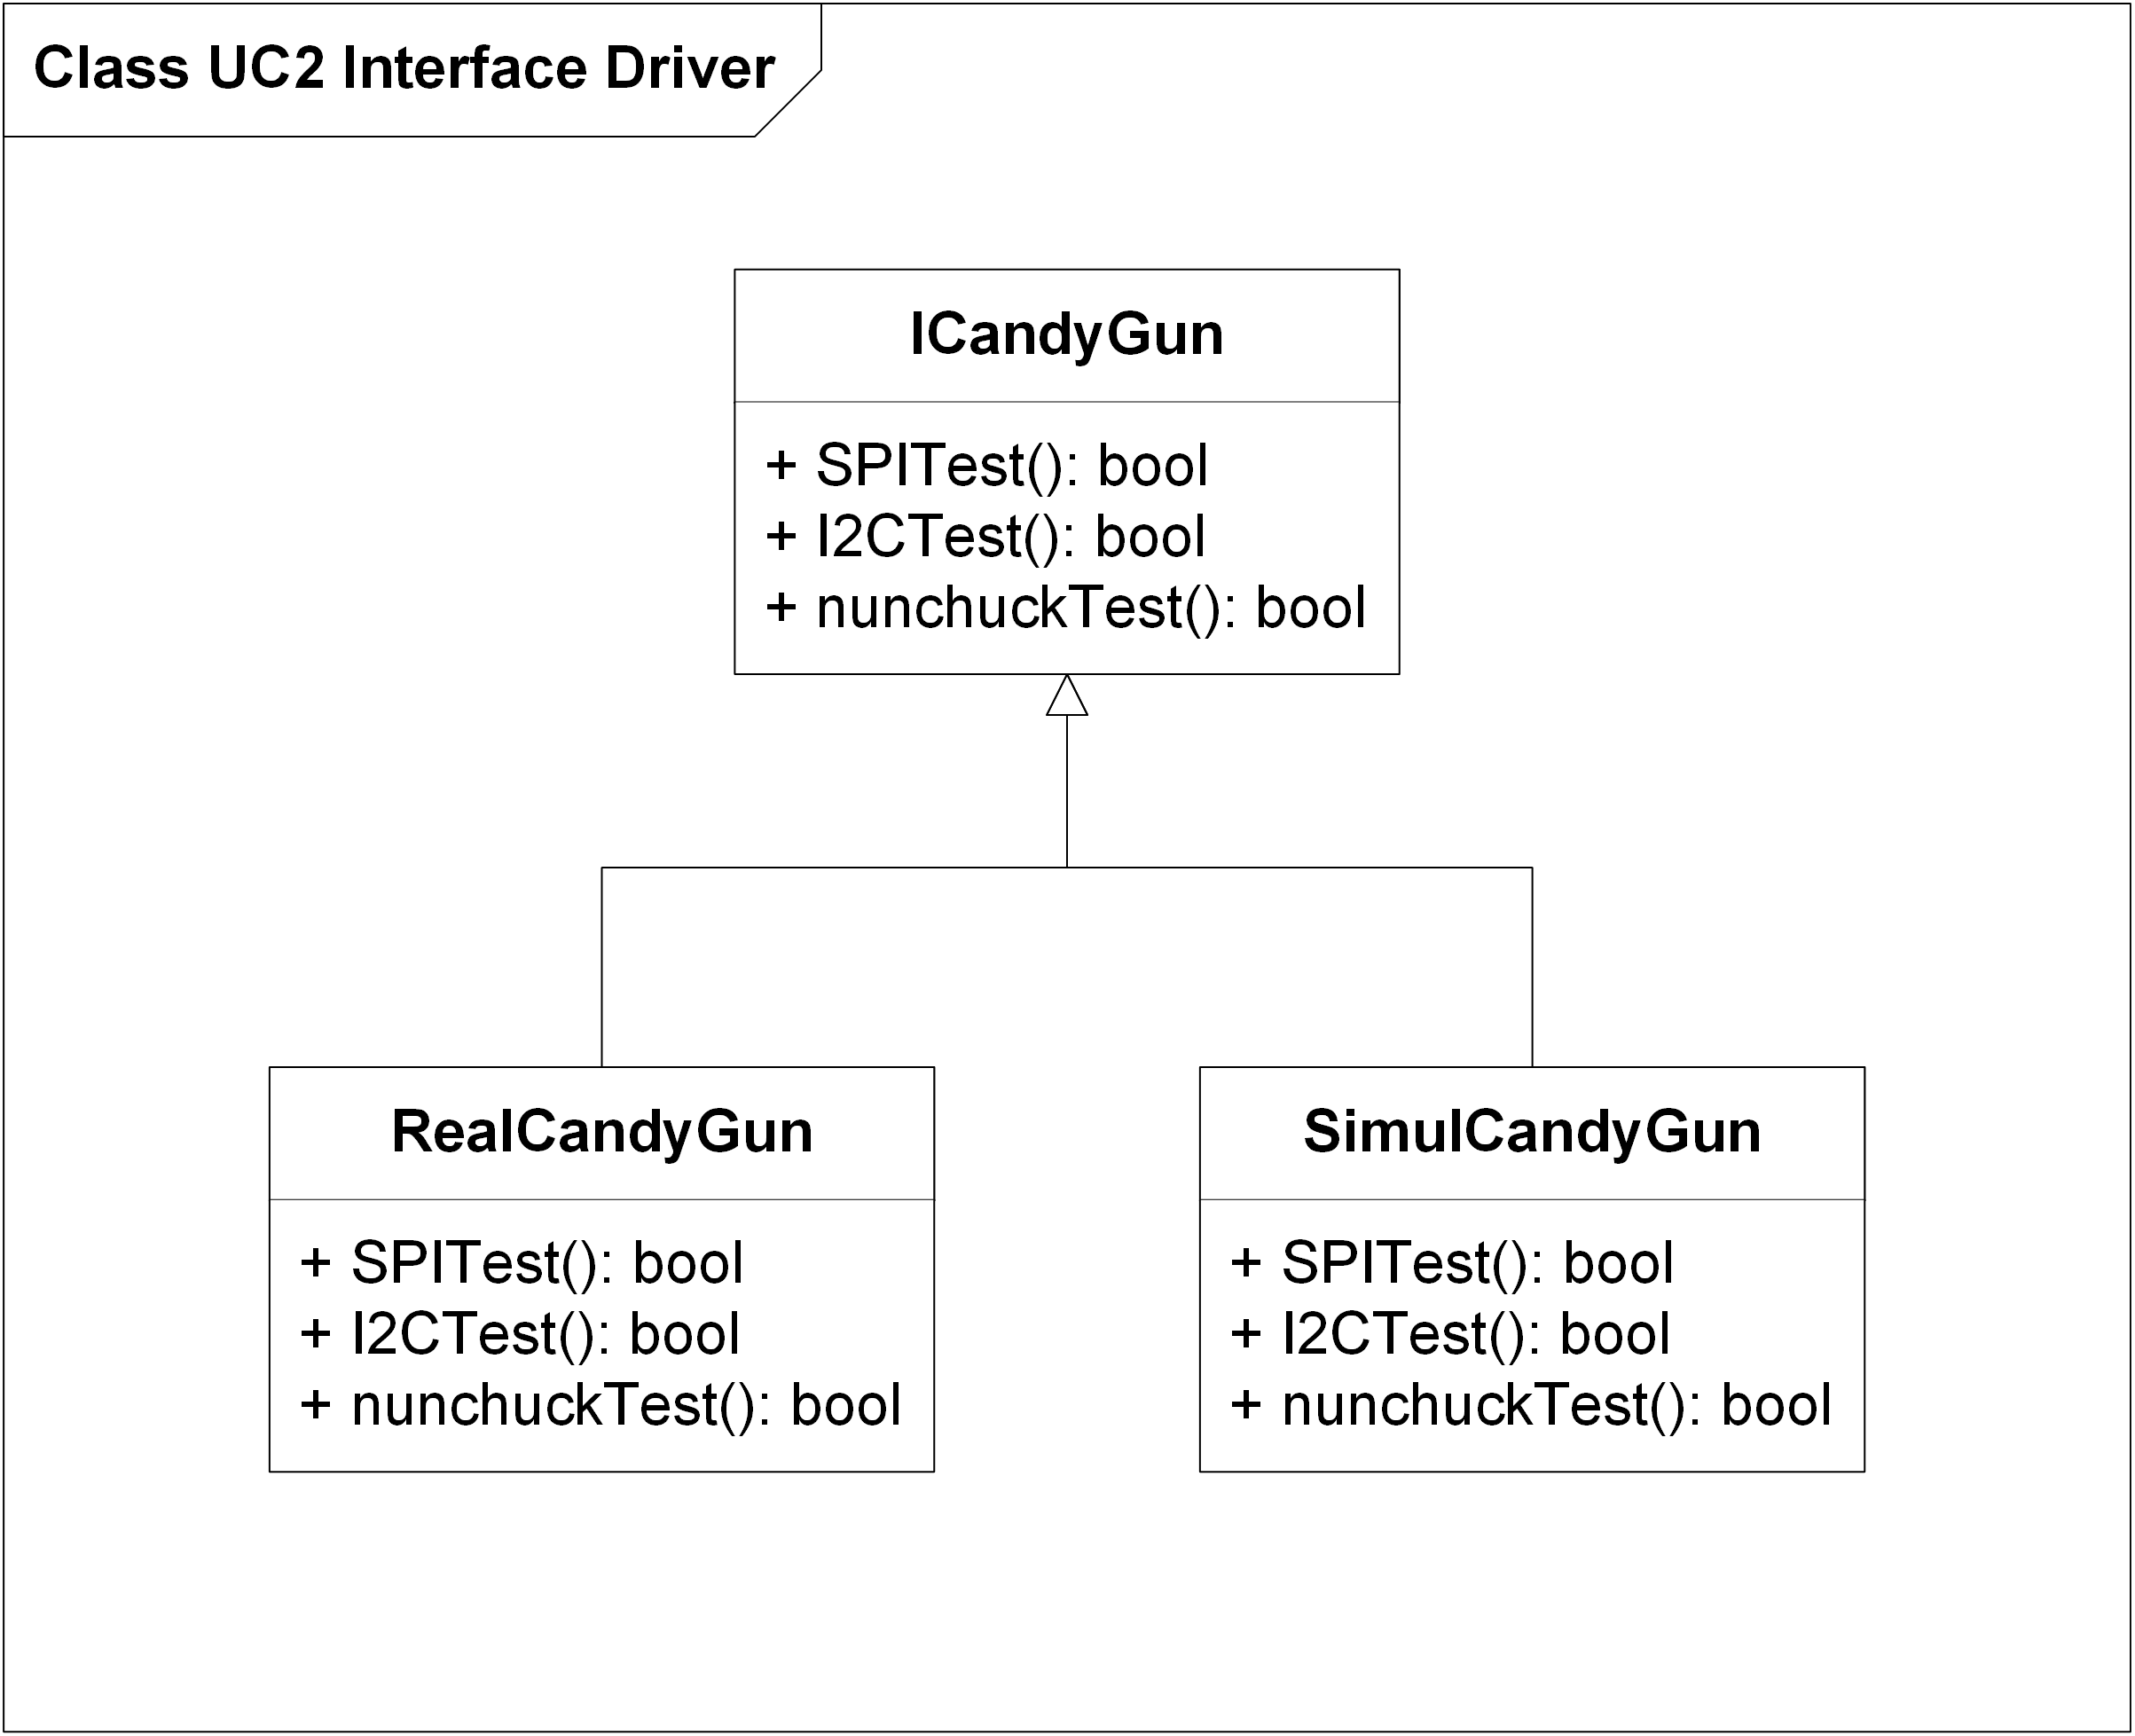
\includegraphics[width=\textwidth]{DesignOgImplementering/images/IdriverKlasseDiagram}
	\caption{Klassediagram for Interface driveren på Devkit8000}
	\label{fig:IDriverKlasseDiagram}
\end{figure}

I det følgende ses tabeller for funktionsbeskrivelser. Funktioner for ICandyGun-klassen er ikke beskrevet, da klassen er abstrakt og ingen af funktionerne dermed er implementeret i klassen. Til gengæld er både funktionerne for SimulCandygun og RealCandyGun beskrevet i hver sin tabel. Bemærk at funktionerne hedder det samme for begge klasser, da de begge er afledte funktioner i et arvehierarki, som det sås på figur \ref{fig:IDriverKlasseDiagram}.  
I tabel \ref{SimulFunktioner} ses funktionsbeskrivelser for SimulCandyGun. 

\begin{table}[H]
	\centering
	% \caption{My caption}
	\label{SimulFunktioner}
	\begin{tabular}{|l|l|}
		\hline
		\textbf{Metode}      & \textbf{Beskrivelse}                                                                                                     \\ \hline
		SPITest(): bool      & Simulerer resultatet af SPI-testen i systemet. \\ Der anvendes rand() til at returnerer et tilfældigt tal mellem 0 og 1.    \\ \hline
		I2CTest(): bool      & Simulerer resultatet af I2C-testen i systemet. \\ Der anvendes rand() til at returnerer et tilfældigt tal mellem 0 og 1.    \\ \hline
		nunchuckTest(): bool & Simulerer resultatet af nuchucktesten i systemet. \\ Der anvendes rand() til at returnerer et tilfældigt tal mellem 0 og 1. \\ \hline
	\end{tabular}
\end{table}


I tabel \ref{realIdriverFunktioner} ses funktionsbeskrivelser for RealCandyGun.

\begin{table}[H]
	\centering
	% \caption{My caption}
	\label{realIdriverFunktioner}
	\begin{tabular}{|l|l|}
		\hline
		\textbf{Metode}      & \textbf{Beskrivelse}                                                                                                                                                                                                                                                                                                                                                                                                                                                           \\ \hline
		SPITest(): bool      & Initierer SPI-test ved at skrive SPI-kommandoen "241" til "dev/candygun", som er den node, der oprettes af Candydriveren. Dernæst indeholder funktionen et delay på 1 sek, for at give SPI-testen tid til at blive udført. Til sidst læser funktionen fra "dev/candygun" og tjekker om den får den korrekte returværdi, "209". Ved korrekt returværdi returnerer funktionen true. Ved fejl returnerer funktionen false.                                                        \\ \hline
		I2CTest(): bool      & Initierer I2C-test ved at skrive I2C-kommandoen "242" til "dev/candygun", som er den node, der oprettes af Candydriveren. Dernæst indeholder funktionen et delay på 1 sek, for at give I2C-testen tid til at blive udført. Til sidst læser funktionen fra "dev/candygun" og tjekker om den får den korrekte returværdi, "210". Ved korrekt returværdi returnerer funktionen true. Ved fejl returnerer funktionen false.                                                        \\ \hline
		nunchuckTest(): bool & Initierer nunchuck-test ved at skrive nunchuck-kommandoen "251" til "dev/candygun", som er den node, der oprettes af Candydriveren. Dernæst indeholder funktionen en whileløkke, som ved at læse fra "dev/candygun" tjekker hvert sekund, om der er trykket på nunchuckknappen. Det ses ved den korrekte returværdi, "211". Ved korrekt returværdi returnerer funktionen true. Ved fejl kører whileløkken igen. Efter 15 sek. uden korrekt værdi, returnerer funktionen false. \\ \hline
	\end{tabular}
\end{table}

\subsection{Brugergrænseflade - WIP}

\begin{figure}[H]
	\centering
	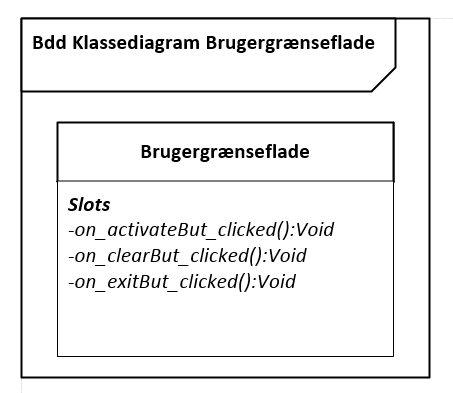
\includegraphics[width=\textwidth]{DesignOgImplementering/images/KlassediagramGUI}
	\caption{Klassediagram for Brugergrænsefladen}
	\label{fig:KlassediagramGUI}
\end{figure}

\subsubsection{Klassebeskrivelse}
\label{sec:stmDescrip}

\noindent\textbf{void on\_activateBut\_clicked()} \newline
Dette slot er startknappen i brugergrænsefladen. Ved tryk bliver knappens signal broadcastet og knappens funktion bliver kørt. Forløbet for dette slot beskrives i figur \ref{fig:stmGUI}. Der skrives til konsolvinduet, derefter testes der på SPITest(). Hvis der returnes true, skrives dette til konsollen og programmet fortsætter til I2CTest(). Hvis der returnes false, skrives dette til konsollen og programmet returnerer til idle-tilstand. Nu testes der på I2CTest(). Hvis der returnes true, skrives dette til konsollen og programmet fortsætter til NunchuckTest(). Hvis der returnes false, skrives dette til konsollen og programmet returnerer til idle-tilstand.
Der testes der på NunchuckTest(). Hvis der returnes true, skrives dette til konsollen, og der skrives at systemtesten er gennemført. Hvis der returnes false, skrives dette til konsollen. Programmeret returnerer til idle-tilstand. \newline

\noindent\textbf{void on\_clearBut\_clicked()} \newline
Dette slot er clearknappen i brugergrænsefladen. Knappens funktionalitet er en clearing af konsol vinduet. \newline

\noindent\textbf{void on\_exitBut\_clicked()} \newline

\begin{figure}[H]
	\centering
	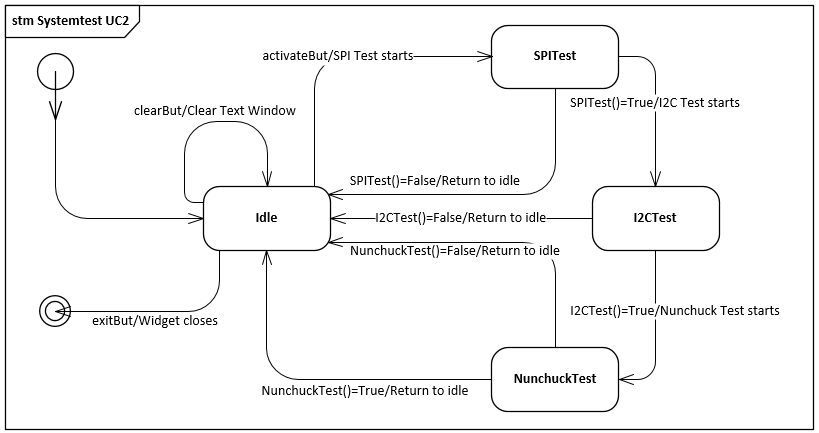
\includegraphics[width=\textwidth]{DesignOgImplementering/images/StateMachineGUIUC2}
	\caption{Statemachine for UC2}
	\label{fig:stmGUI}
\end{figure}


\section{PSoC Software}

%\subsection{PSoC Software}
De følgende klassediagrammer på figur \ref{figure:klassediagramPSoC0} og \ref{figure:klassediagramPSoC1} giver et overblik over hvilke klasser der bliver gjort brug af på PSoC0 og PSoC1. De efterfølgende afsnit vil beskrive klasserne og deres funktioner.

\begin{figure}[H]
	\centering
	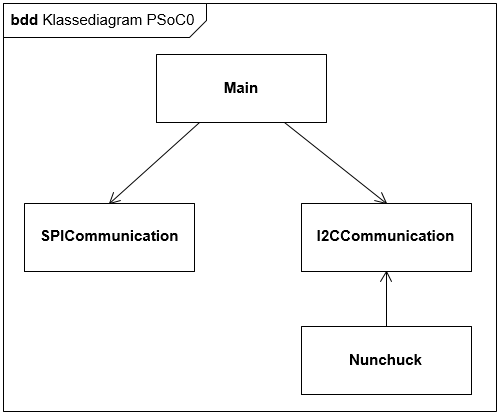
\includegraphics[width=.7\textwidth]{DesignOgImplementering/images/PSoC0KlassediagramOversigt}
	\caption{Klassediagram oversigt for PSoC0}
	\label{figure:klassediagramPSoC0}
\end{figure}

\begin{figure}[H]
	\centering
	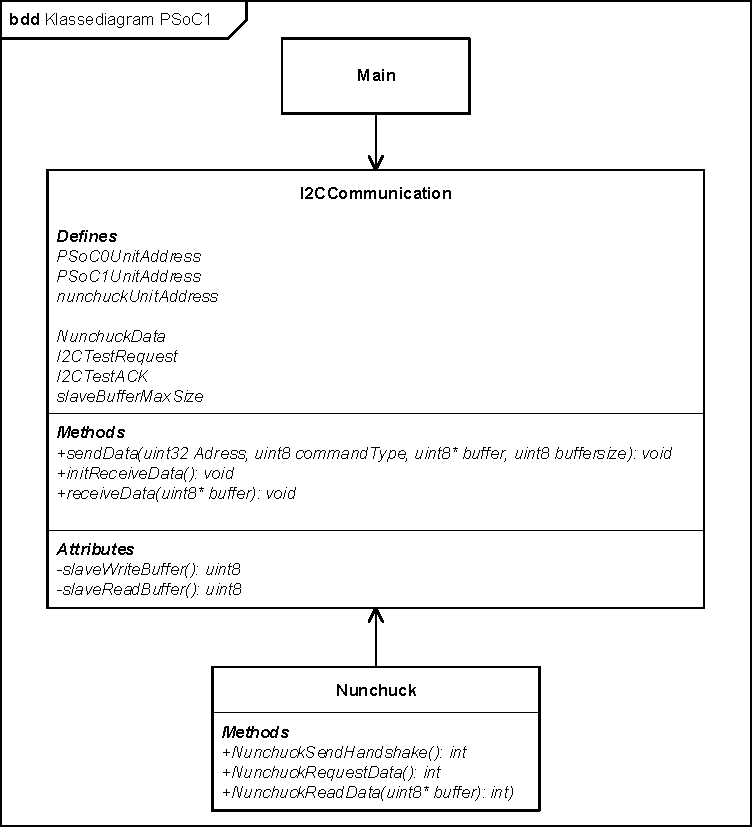
\includegraphics[width=.7\textwidth]{DesignOgImplementering/images/PSoC1KlassediagramOversigt}
	\caption{Klassediagram oversigt for PSoC1}
	\label{figure:klassediagramPSoC1}
\end{figure}

\subsection{SPI - PSoC}
I dette afsnit vil softwaren der specifikt omhandler SPI-kommunikationen mellem PSoC0 og DevKit8000 blive beskrevet. Dette gøres vha. et klassediagram og klassebeskrivelser

\subsubsection{Klassediagram}
På figur \ref{figure:KlassediagramSPICommunication} ses klassediagrammet over SPICommunication klassen.

\begin{figure}[H]
	\centering
	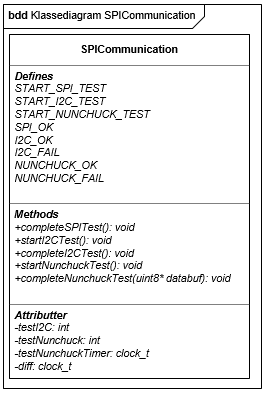
\includegraphics[]{DesignOgImplementering/images/SPICommunication}
	\caption{Klassediagram over klassen SPICommunication}
	\label{figure:KlassediagramSPICommunication}
\end{figure}
\subsubsection{Klassebeskrivelser}
I dette afsnit vil klassens metoder og defines blive beskrevet.
\newline

\noindent\textbf{void completeSPITest()} \newline
Denne metode gemmer \textit{SPI\_OK} i PSoC'ens SPI-transfer buffer. \newline

\noindent\textbf{void completeI2CTest()} \newline
Denne metode gennemfører I2C-Testen. Dette gøres ved at der sendes en besked til alle enheder på I2C-nettet, og hvis der ikke registreres nogen fejl på denne besked, bliver \textit{I2C\_OK} gemt i PSoC'ens SPI-transfer buffer. Registreres der en fejl, bliver \textit{I2C\_FAIL} gemt i SPI-transfer buffer. \newline

\noindent\textbf{void completeNunchuckTest(uint8* databuf)} \newline
Denne metode gennemfører Nunchuck-testen. Dette gøres ved at der startes en timer på 6 sekunder. Hvis der sker et tryk på 'Z'-knappen på nunchucken indenfor disse 6 sekunder, vil \textit{NUNCHUCK\_OK} blive gemt i SPI-transfer bufferen. Hvis der ikke registreres nogen tryk inden for de 6 sekunder, er det \textit{NUNCHUCK\_FAIL} der gemmes.\newline

I klassediagrammet er der beskrevet en række "Defines". Disse defines bruges i klassen som unikke ID'er der indikerer om en test er gennemført OK eller om den er fejlet.

\subsubsection{SPI Indstillinger på PSoC}
I forbindelse med SPI forbindelsen i systemet, skal der sættes nogle indstillinger på PSoC0, idét at denne kommunikerer med Devkittet via SPI. 
PSoC'en sættes som en slave, idét at det er Devkittet der aflæser og skriver til PSoC0.
SCLK sættes til CPHA=1 og CPOL=1. Disse er valgt arbitrært, dog ud fra den forudsætning, at de skal stemme overens med indstillingerne på Devkittet, idét disse indstillinger beskriver hvornår databit aflæses/sættes i forhold til clock'en. 
'Data Rate' sættes til 1Mbps, da dette er en sikker/stabil overførselshastighed. Igen skal denne indstilling være ens for PSoC og Devkit.
Den sidste indstilling der sættes, er 'transfer' og 'read' buffer size. Disse er valgt til at være 8-bit, da projektets SPI kommunikationsprotokol ikke har brug for størrere datamængder. Igen skal denne indstilling være ens for både SPI-master og slave. 

\subsection{I2CCommunication}
I dette afsnit vil softwaren der omhandler I2C-kommunikation blive beskrevet. Dette inkluderer et klassediagram,  klassebeskrivelser og indstillingerne for I2C kommunikationen på PSoC'en.

\subsubsection{Klassediagram}
På figur \ref{figure:klassediagramI2CCommunication} ses klassediagrammet for I2CCommunication. 
\begin{figure}[H]
	\centering
	%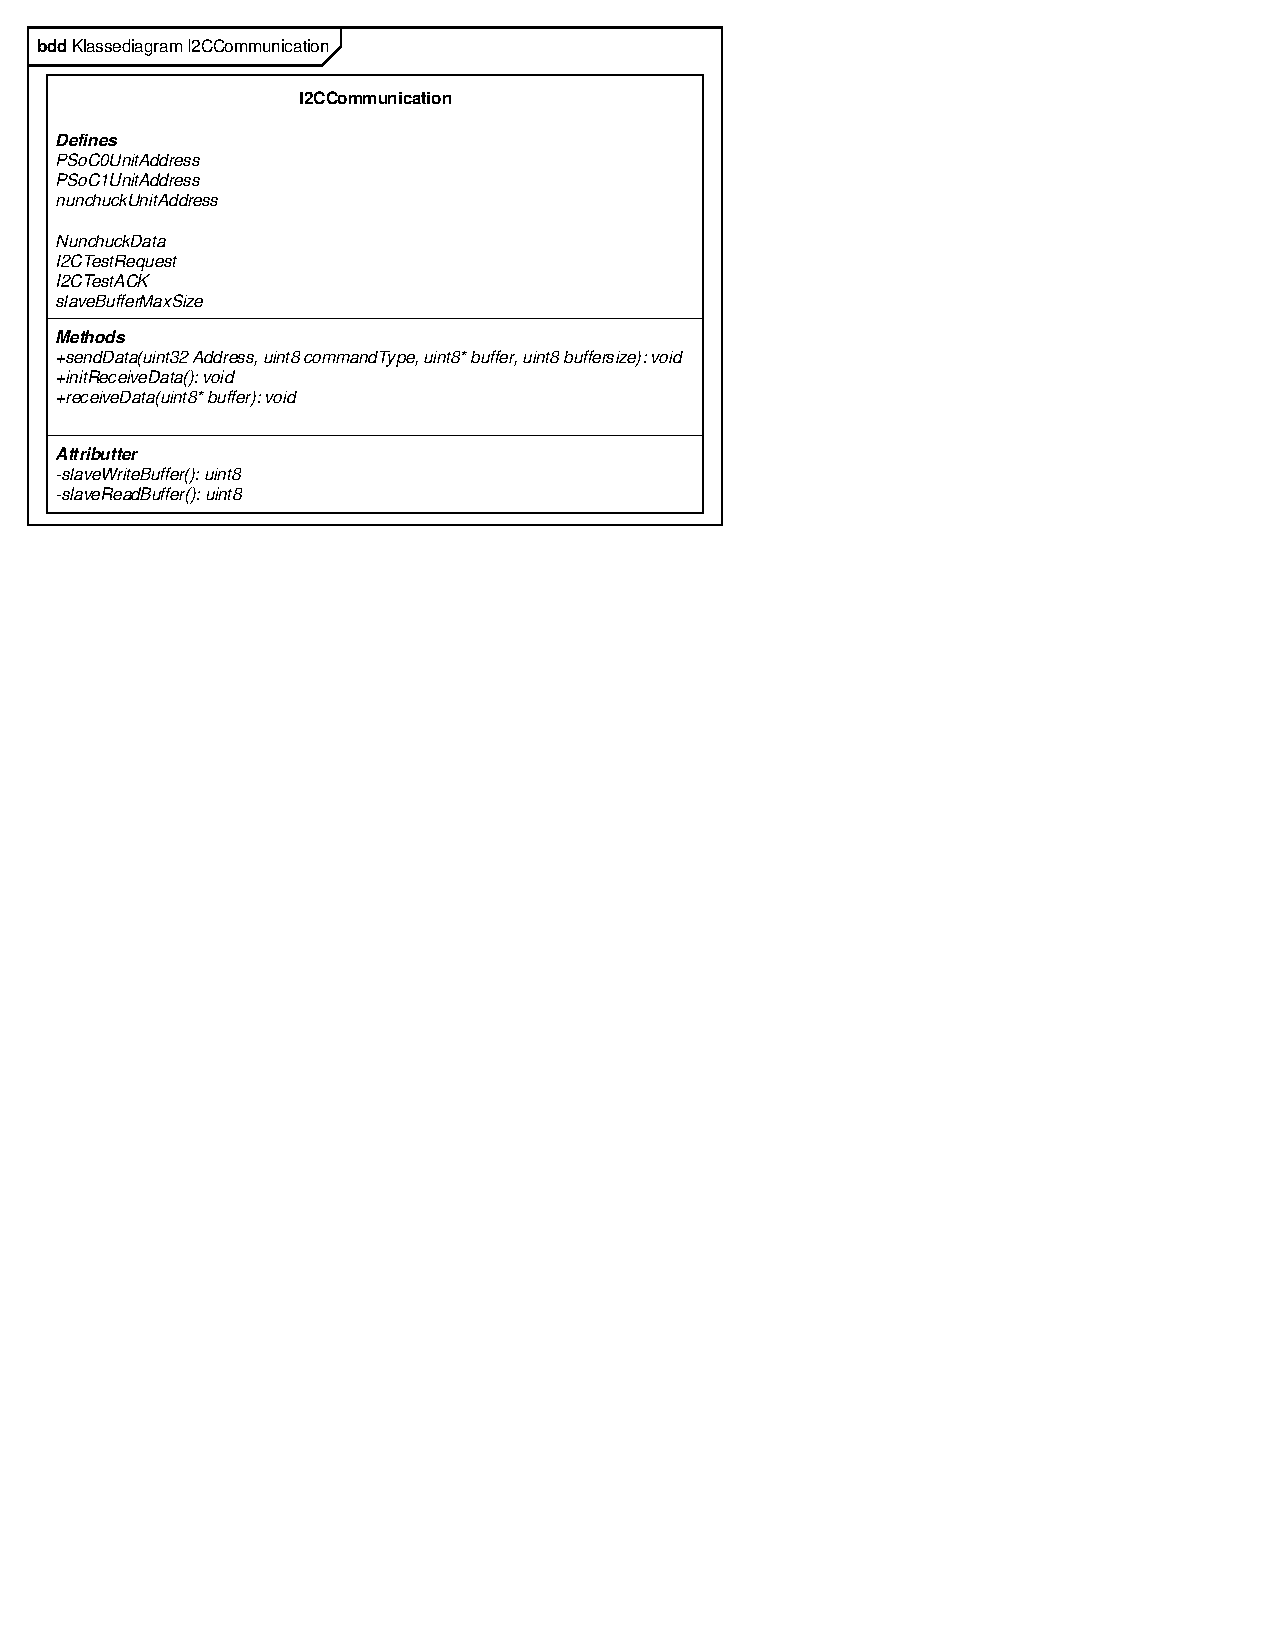
\includegraphics[width=0.9\textwidth, trim={0 19cm 9cm 0},clip]{DesignOgImplementering/images/I2CCommunication.pdf}
	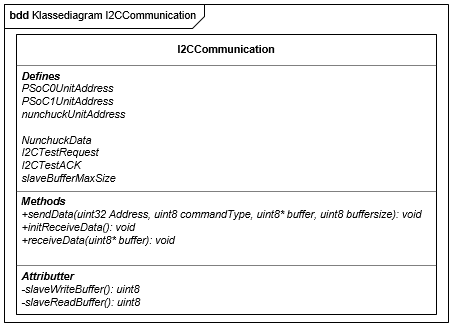
\includegraphics[]{DesignOgImplementering/images/I2CCommunication}
	%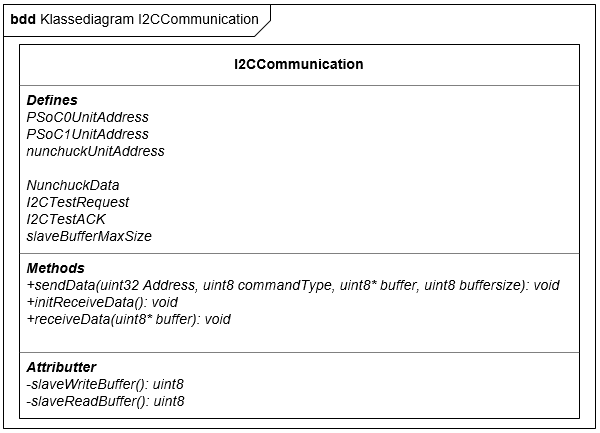
\includegraphics[width =0.9\textwidth]{DesignOgImplementering/images/I2CCommunication2}
	\caption{Klassediagram for I2CCommunication klassen}
	\label{figure:klassediagramI2CCommunication}
\end{figure}

\subsubsection{Klassebeskrivelser}
Som det ses på klassediagrammet figur \ref{figure:klassediagramI2CCommunication} indeholder klassen flere metoder. Disse metoder blive beskrevet her.\newline

\noindent\textbf{void sendData(uint8 Address, uint8 commandType, uint8* buffer, uint8 buffersize)}\newline
Denne metode sender, via PSoC Creators I2C-API, den data der ligger i "buffer" af kommandotypen "commandType" til slaven med adressen "Address". \newline

\noindent\textbf{void initReceiveData()} \newline 
Denne metode initialiserer de to buffers (slaveWrite og slaveRead) der kræves på en I2C-slave, for at kunne gøre bruge af PSoC Creator's I2C-API. \newline

\noindent\textbf{void receiveData(uint8* buffer)}\newline
Denne metode venter på at slaveRead bufferen er blevet fyldt. Når dette er sket, bliver slaveRead bufferen kopieret over i "buffer".

\subsubsection{I2C indstillinger på PSoC}
I forbindelse med at have en I2C forbindelse på PSoC'en, er der et par indstillinger der skal sættes. Hver PSoC der gør brug af I2C, sættes til at være en "Multi-master-slave". Dette gøres for at alle I2C enheder kan gøre brug af "I2CCommunication" klassen, idét at denne indeholder funktioner for både master og slave. 
En anden vigtig indstilling er I2C bussens 'Data Rate'. Denne er fra PSoC creators side sat til 100kbps som standard, hvilket er en passende hastighed for dette projekt.
En hver enhed på I2C nettet skal også have en adresse. En tabel for adressefordelingen ses på tabel \ref{table:I2CAddress}


\subsection{Nunchuck}
I dette afsnit vil softwaren der specifikt omhandler kommunikationen mellem PSoC0 og Nunchucken blive beskrevet. Dette gøres vha. et klassediagram og klassebeskrivelser.

\subsubsection{Klassediagram}
På figur \ref{figure:NunchuckKlassediagram} ses klassediagrammet for Nunchuck klassen.

\begin{figure}[H]
	\centering
	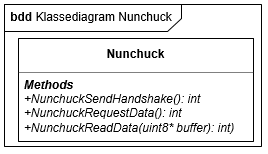
\includegraphics[]{DesignOgImplementering/images/nunchuck}
	\caption{Klassediagram for klassen Nunchuck}
	\label{figure:NunchuckKlassediagram}
\end{figure}

\subsubsection{Klassebeskrivelser}
Metoderne fra klassediagrammet figur \ref{figure:NunchuckKlassediagram} vil blive beskrevet i dette afsnit.

\noindent\textbf{int NunchuckSendHandshake()}\newline
Denne metode sender et "handshake" (Se dokumentationen afsnit \textbf{INSERT AFSNIT HER \#ref}) til Nunchuck enheden. Handshaket bruges til at "parre" PSoC'en med nunchucken. Metoden returnerer et '0' hvis der opstår en fejl. \newline

\noindent\textbf{int NunchuckRequestData()}\newline
Denne metode sender et 0x00 til nunchuck'en, og derved beder nunchuck'en om at klargøre data til overførsel. Metoden returnerer et '0' hvis der opstår en fejl. \newline

\noindent\textbf{int NunchuckreadData(uint8* buffer)}\newline
Denne metode bruger PSoC Creator's I2C-API til at læse data fra nunchuck'en (data der blev klargjort fra NunchuckRequestData()). Disse data bliver derefter dekrypteret og gemt i "buffer", så de bliver tilgængelige uden for metodens scope. \newline

I klassediagrammet er der en sektion kaldet "Defines". Disse Defines bruges i implementeringen til forskellige formål. \textit{PSoC0UnitAddress, PSoC1UnitAddres} og \textit{nunchuckUnitAddress} bruges til at definere adresserne for I2C-nettets slaver. \textit{NunchuckData, I2CTestRequest} og \textit{I2CTestACK} er kommando typer der bruges til at bestemme hvilken kommando type der er blevet sendt/modtaget, og hvor mange bytes der skal forventes at være gemt i databufferen (Se dokumentationen afsnit \textbf{INDSÆT REFERENCE TIL DOKUMENTATIONAFSNIT \#ref}) 

\subsection{Rotationsbegrænsning}
I forbindelse med begrænsning af motorens rotation er der nogle indstillinger der skal sættes. ADC'en skal indstilles til at gøre brug af en kanal i single mode, da der ét inputsignal fra potentiometret og denne skal bestemmes i forhold til stel. For at styre motorens bevægelse i et interval er følgende algoritme implementeret.

\begin{figure}[H]
	\centering
	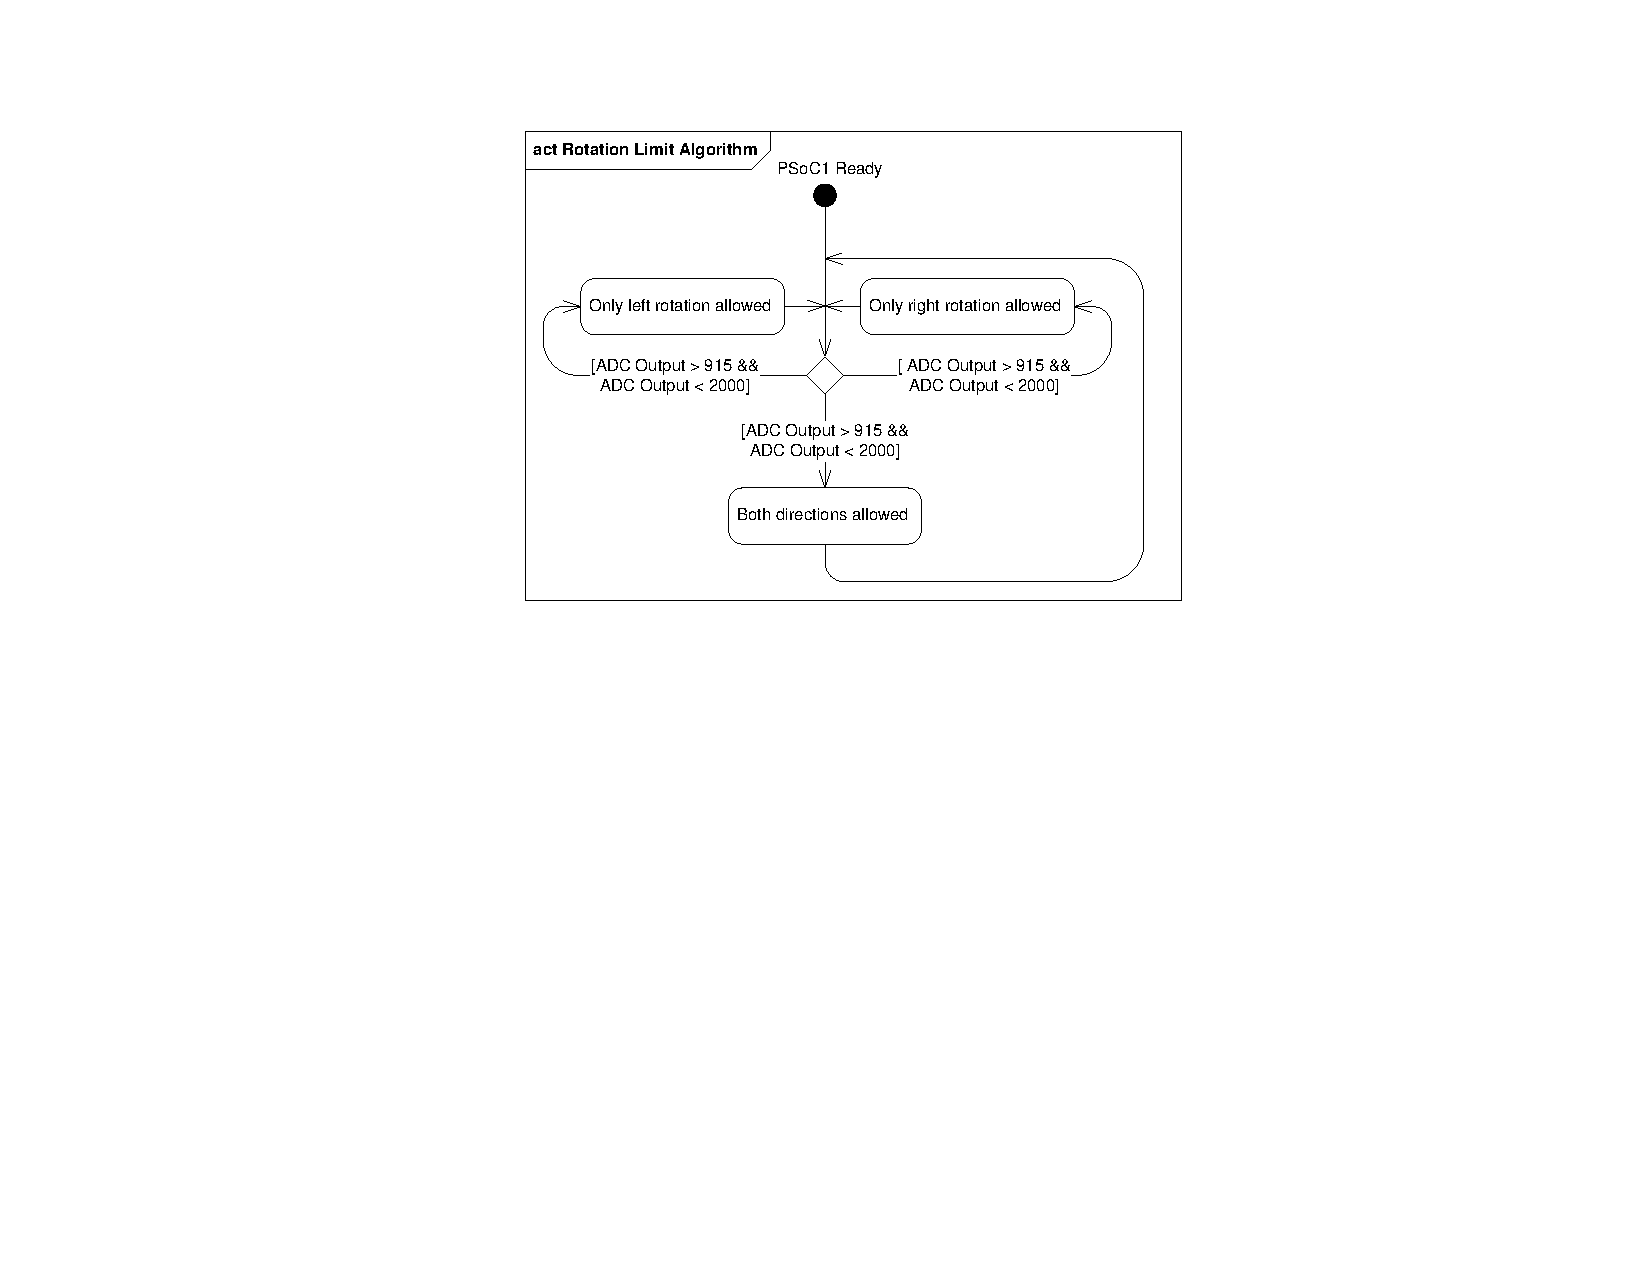
\includegraphics[width=\textwidth]{DesignOgImplementering/images/rotationalgorithm}
	\caption{Aktivitetsdiagram for rotationsbegrænsningsalgortimen}
	\label{fig:rotation}
	
\end{figure}

\noindent På figur \ref{fig:rotation} ses et aktivitetsdiagram for algoritmen for rotationsbegrænsning. Der er fastsat to værdier for ydergrænser. Når motoren bevæger sig udover ydergrænserne, blokeres motoren for den givne retning indtil motoren er tilbage i intervallet. 

\subsection{Motorstyring}
Til styring af motorene gøres der brug af fire PWM blokke, to til styring af X-aksen og to til styring af Y-aksen. Disse PWM blokke er indstillet med en clock frekvens på 3MHz. Til styring af motorene er følgende algoritme implementeret. 
\begin{figure}[H]
	\centering
	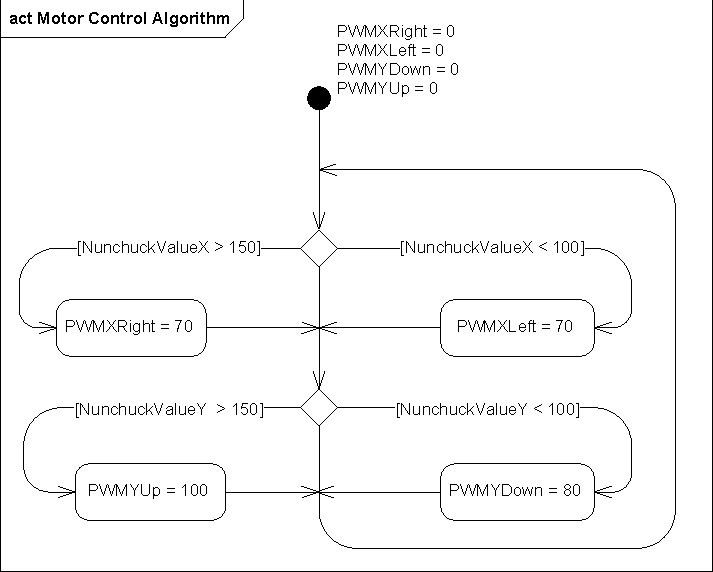
\includegraphics[scale=0.8]{DesignOgImplementering/images/motorcontrolalgorithm}
	\caption{Aktivitetsdiagram for motorstyringsalgortimen}
	\label{fig:motorstyringal}
\end{figure}

\noindent På figur \ref{fig:motorstyringal} ses aktivitetsdiagrammet for motorstyringsalgoritmen. Der ses at retningensignalerne bestemmes ud fra Wii-Nunchuck'ens inputværdier fra X- og Y-aksen.

\section{Afkodning af Wii-Nunchuck Data Bytes}
Aflæste bytes fra Wii-Nunchuck - indeholdende tilstanden af knapperne og det analoge stick - er kodet når de oprindeligt modtages via I2C bussen. Disse bytes skal altså afkodes før deres værdier er brugbare. Afkodningen af hver byte sker ved brug af følgende formel:

\textit{AfkodetByte = (AflæstByte XOR 0x17) + 0x17}

Fra formlen kan det ses at den aflæste byte skal \textit{XOR}'s (Exclusive Or) med værdien 0x17, hvorefter dette resultat skal adderes med værdien 0x17.

\section{Kalibrering af Wii-Nunchuck Analog Stick}
De afkodede bytes for Wii-Nunchuck's analoge stick har definerede standardværdier for dets forskellige fysiske positioner. Disse værdier findes i tabel \ref{tabel:WiiNunchuckStickPositioner}

\begin{table}[H]
	\centering
	\begin{tabular}{|l|l|}
		\hline
		X-akse helt til venstre & 0x1E \\ \hline
		X-akse helt til højre   & 0xE1 \\ \hline
		X-akse centreret        & 0x7E \\ \hline
		Y-akse centreret        & 0x7B \\ \hline
		Y-akse helt frem        & 0x1D \\ \hline
		Y-akse helt tilbage     & 0xDF \\ \hline
	\end{tabular}
	\caption{Standardværdier for fysiske positioner af Wii-Nunchuck's analoge stick}
	\label{tabel:WiiNunchuckStickPositioner}
\end{table}

I praksis skal de afkodede værdier for det analoge stick kalibreres, da slør pga. brug gør at de ideale værdier ikke rammes. 

I projektet er de afkodede værdier for det analoge stick kalibreret med værdien -15 (0x0F i hexadecimal), altså ser den endelige formel for afkodning samt kalibrering således ud:

\textit{AfkodetByte = (AflæstByte XOR 0x17) + 0x17 - 0x0F}

\section{Hardwaredesign}
På baggrund af BDD'et er der fundet følgende hardwareblokke, der skal udarbejdes: 
\begin{itemize}
	\item Motorstyring
	\item Tre motorer
	\item Affyringsmekanisme 
\end{itemize}
Disse beskrives i de følgende afsnit. 

\subsubsection{Motor}
Der er valgt at bruge en DC-motor i alle tre tilfælde. De to motorer skal bruges til at styre kanonen i to retninger, og den sidste skal bruges i affyringsmekanismen. 

\subsection{Motorstyring}
Til at styre de tre motorer er der bygget en H-bro, der skal bruges i tre eksemplarer. To af disse motorer skal kunne styre kanonen, så den ene gør at den kan køre op og ned, og den anden gør, at den kan køre fra side til side. Den tredje skal bruges til at styre affyringsmekanismen. 

\subsubsection{H-bro}
Der blev først designet en H-bro, som bestod af to N-MOSFET's af typen IRLZ44 og to P-MOSFET's af typen ZVP3306. Denne kan ses i bilaget. Det viste sig dog, at den P-MOSFET, der var brugt, var for svag til at kunne trække den strøm, som motoren skulle bruge, hvilket betød, at den blev brændt af. Derfor blev denne H-bro modificeret, så de to P-MOSFET's blev udskiftet med to MOSFET's af typen IRF9Z34N, der kan trække en større strøm. 

\begin{figure}[H]
	\centering
	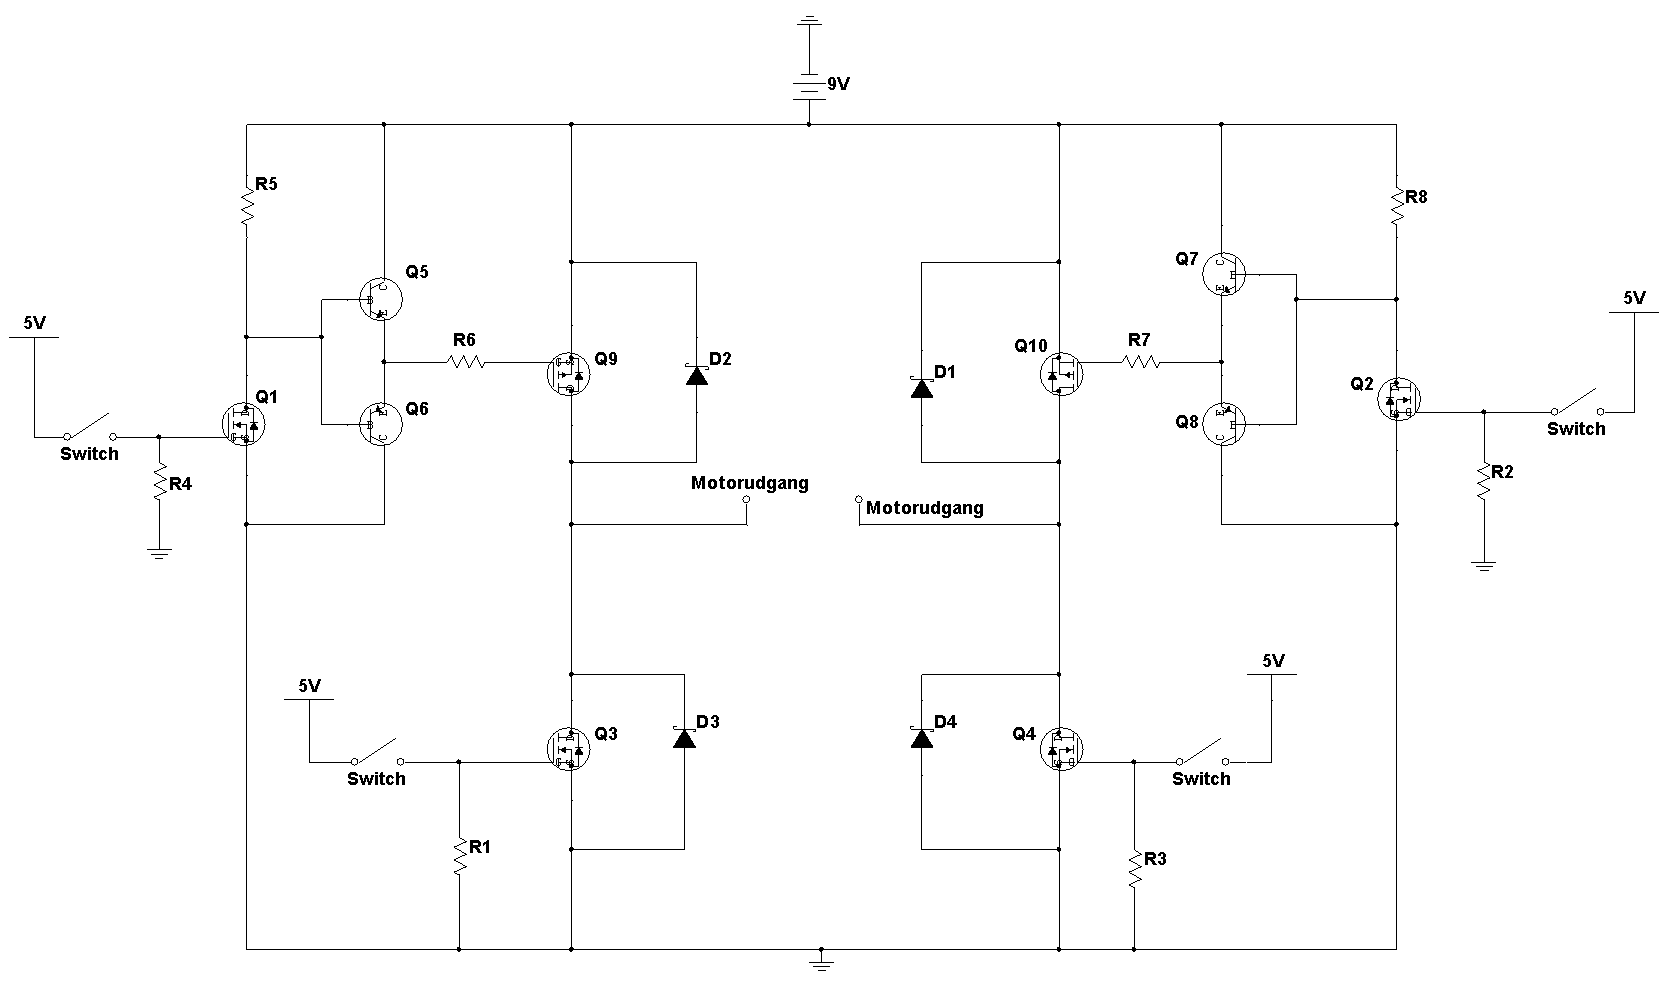
\includegraphics[width=\textwidth]{DesignOgImplementering/images/H-bro}
	\caption{Kredsløb for H-bro}
	\label{fig:hbro}
	\end{figure}
	

\begin{table}[H]
	\centering
	\begin{tabular}{|l|l|l}
		\cline{1-2}
		Betegnelse 	& Komponent 	          	 &  \\ \cline{1-2}
		VCC        	& 5V                         &  \\ \cline{1-2}
		Q1   		& IRLZ44(mosfet N-Channel)   &  \\ \cline{1-2}
		Q2   		& IRLZ44(mosfet N-Channel)   &  \\ \cline{1-2}
		Q3   		& IRLZ44(mosfet N-Channel)   &  \\ \cline{1-2}
		Q4   		& IRLZ44(mosfet N-Channel)   &  \\ \cline{1-2}
		Q5   		& BC547                      &  \\ \cline{1-2}
		Q6   		& BC557                      &  \\ \cline{1-2}
		Q7   		& BC547                      &  \\ \cline{1-2}
		Q8   		& BC557                      &  \\ \cline{1-2}
		Q9   		& IRF9Z34N(mosfet P-Channel) &  \\ \cline{1-2}
		Q10  		& IRF9Z34N(mosfet P-Channel) &  \\ \cline{1-2}
		R1   		& 10k$\Omega$                &  \\ \cline{1-2}
		R2   		& 10k$\Omega$                &  \\ \cline{1-2}
		R3   		& 10k$\Omega$                &  \\ \cline{1-2}
		R4   		& 10k$\Omega$                &  \\ \cline{1-2}
		R5   		& 10k$\Omega$                &  \\ \cline{1-2}
		R6   		& 100$\Omega$                &  \\ \cline{1-2}
		R7   		& 100$\Omega$                &  \\ \cline{1-2}
		R8   		& 10k$\Omega$                &  \\ \cline{1-2}
		D1   		& IN5819                     &  \\ \cline{1-2}
		D2   		& IN5819                     &  \\ \cline{1-2}
		D3   		& IN5819                     &  \\ \cline{1-2}
		D4   		& IN5819                     &  \\ \cline{1-2}
	\end{tabular}
	\caption{Komponentbetegnelser på H-bro 5}
	\label{my-label}
\end{table}


\subsubsection{MOSFET'er}
Til at styre motoren er der bygget en H-bro, som består af fire mosfet, hvor to af dem er af typen IRF9Z34N (mosfet P-channel, som er Q9 og Q10 på figur \ref{fig:hbro}) og de to andre mosfet er af typen IRLZ44 (mosfet N-Channel, som er Q3 og Q4 på figur\ref{fig:hbro}). Det er valgt at bruge mosfet for at kunne styre H-broen, da det ved denne er muligt at lukke og åbne for spændingen, og de bliver styret af spænding, i forhold til transistorer, som bliver styret af strøm. 

\begin{itemize}
\item MOSFET N-kanal\\
	Der er i denne H-bro brugt en N-kanals-MOSFET af typen IRLZ44. Denne MOSFET skal bruges til at trække strømmen fra den tilsvarende P-MOSFET til stel, så motoren kan begynde at køre. Det sker, når der kommer 5V ind på gate-benet. 
	\\MOSFET'en fungerer på den måde, at når der kommer positiv spænding ind på gate-benet åbner den, så der kommer forbindelse til stel og når der kommmer 0V ind på dette lukker den igen. 
	
	\begin{figure}[H]
		\centering
		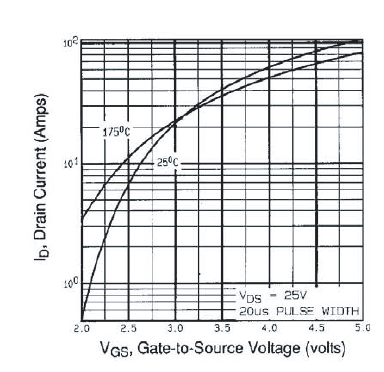
\includegraphics[width=\textwidth]{DesignOgImplementering/images/grafn}
		\caption{Gate-to-Source Voltage REFERENCE TIL DATABLAD HER!!!!}
		\label{fig:mosfetn}
	\end{figure}
	
	På figur \ref{fig:mosfetn} ses det, at når der er en gate-to-source-spænding på 5V, vil der MOSFET'en kunne klare, at der løber en strøm på op til 100A i følge datablad \textbf{\#ref Reference til datablad}. Det vil altså ikke komme til at påvirke motoren, da denne kun kan trække en strøm på cirka 0,35A. 
	
\item MOSFET P-kanal \\
	Der er valgt at bruge en P-MOSFET af typen IRF9Z34N. Denne MOSFET skal bruges til at trække de 12V ned til motoren, så denne kan køre. Samtidig sørger den for, at de 12V ikke løber ned til motoren så længe, der ikke er negativ spænding på gate-benet. 
	Denne type MOSFET kan trække en strøm på 6,7A ifølge databladet \textbf{\#ref Reference til datablad}. Det vil altså ikke komme til at påvirke motoren, da den kun kan trække en strøm på cirka 0,35A. 
	
	For at der kan løbe spænding igennem IRF9Z34N, skal den have en negativ spænding for at åbne og en spænding på over 0V for at lukke. 
		
	\begin{figure}[H]
		\centering
		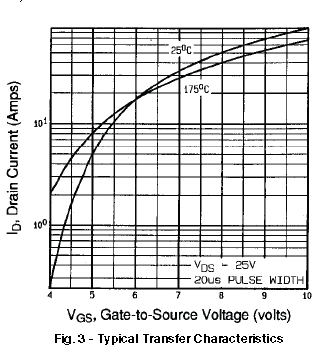
\includegraphics[width=\textwidth]{DesignOgImplementering/images/grafp}
		\caption{Gate-to-Source Voltage REFERENCE TIL DATABLAD HER!!!!}
		\label{fig:mosfetp}
	\end{figure}
	
	På figuren \ref{fig:mosfetp} ses det, at når der er en gate-to-source-spænding på 5V, vil derr kunne løbe en strøm på omkring 5A igennem MOSFET'en, hvilket er mere end nok til at få motoren til at køre. 
	
\end{itemize}

\subsubsection{Dioder}
Over fire af mosfetene (Q9, Q10, Q3 og Q4) som set på figur \ref{fig:hbro} er der sat en diode af typen IN5819. Den skal fungere som beskyttelse af de fire mosfet (Q9, Q10, Q3 og Q4). Det, de gør, er, at de sikrer, at den spænding, som er tilbage i motoren, når man lukker for mosfetene, ikke løber tilbage ind i mosfetene og brænder dem af.

\subsubsection{Modstande}
\begin{itemize}
	\item Pull down modstande:\\
	Der er blevet brugt fire pull-down-modstande (R1, R2, R3 og R4 som set på figur \ref{fig:hbro}). Disse sørger for, at signalet vil blive holdt lavt, når der ikke er trykket, så dette ben ikke står og flyver, så det kan komme til at åbne en mosfet ved en fejl og derved kommer til at brænde en mosfet eller motoren af. Der er valgt en modstand på 10 kOhm, hvilket betyder, at den er lille nok til at trække de små spændinger ned, når der ikke er trykket, og den stor nok til at spændingen ikke løber derned, når der er trykket. 
	\item Andre modstande
	\begin{itemize}
		\item R6 og R7\\
			Grunden til, at R6 og R7(på figur \ref{fig:hbro}), er der, er for at sikre, at transistorernes Absolute Maximum Ratings omkring strømmen, som ikke må overstige 100mA ifølge databladet. (tjek lige om det er rigtig)
		
			
			\begin{displaymath}
			\frac {9V}{100mA} 	=90\Omega
			\end{displaymath}
			Der blev sat en 100$\Omega$ i stedet for at være sikker på at der ikke var noget som blev brændt af
		\item R5 og R8\\
			Grunden til at R5 og R8(kan ses på figur \ref{fig:hbro}) er sat ind i kredsløbet er, at der ifølge databladet kun kan løbe en strøm på omkring 30A igennem den N-MOSFET, der er brugt, Vgs er 10V. Da Vgs kun er sat til 5V, vil MOSFET'en altså ikke kunne klare en alt for stor strøm. Derfor er R5 og R8 sat ind for at forhindre, at MOSFET'en ikke brænder af.
			 \begin{displaymath}
			 \frac {9V}{30A} 	=0.3\Omega
			 \end{displaymath}
			 0.3$\Omega$ alt for lidt, så der blev prøvet end til der blev fundet en som virkerede og det var 10K$\Omega$
	\end{itemize}

\end{itemize}

\subsubsection{Transistorer}
\begin{itemize}
	\item Q5 og Q7(kan ses på figur \ref{fig:hbro})
	Disse transistorer sidder i kredsløbet, fordi det tager tid for P-MOSFET'en at blive opladt helt, på grund af kondensator effekt imellem benene på mosfet'en, for ellers ville den tag for lang tid om at åbne helt. Det hjælper den disse transistorer til med. 
	
	\item Q6 og Q8(kan ses på figur \ref{fig:hbro})
	Disse to transistorer sidder der for at hjælpe med at lukke P-MOSFET'en igen. Inden Q5 og Q7 blev sat ind tog det tid for at lukke P-MOSFET'en, men da de to blev sat ind, kunne de hjælpe til med at aflade mosfet'ene hurtigere. Derfor sidder de der, for at IRF9Z34N kan lukke hurtigt. 
\end{itemize}

\subsubsection{Rotationsbegrænsning}
Platformen, som styres af motoren, må ikke kunne rotere 360 \(\deg\). Dette ses kravspecifikationen \textbf{\#ref Reference til kravspecikation (ikke-funktionelle krav)}. For at begrænse motorens bevægelse, anvendes et potentiometer samt en ADC. Når motoren bevæger sig, ændres potentiometerets modstandsværdi, og dermed ændres spændingsniveauet. På figur \ref{fig:opstillingADC} ses den endelige opstilling af rotationsbegrænsningen.

\begin{figure}[H]
	\centering
	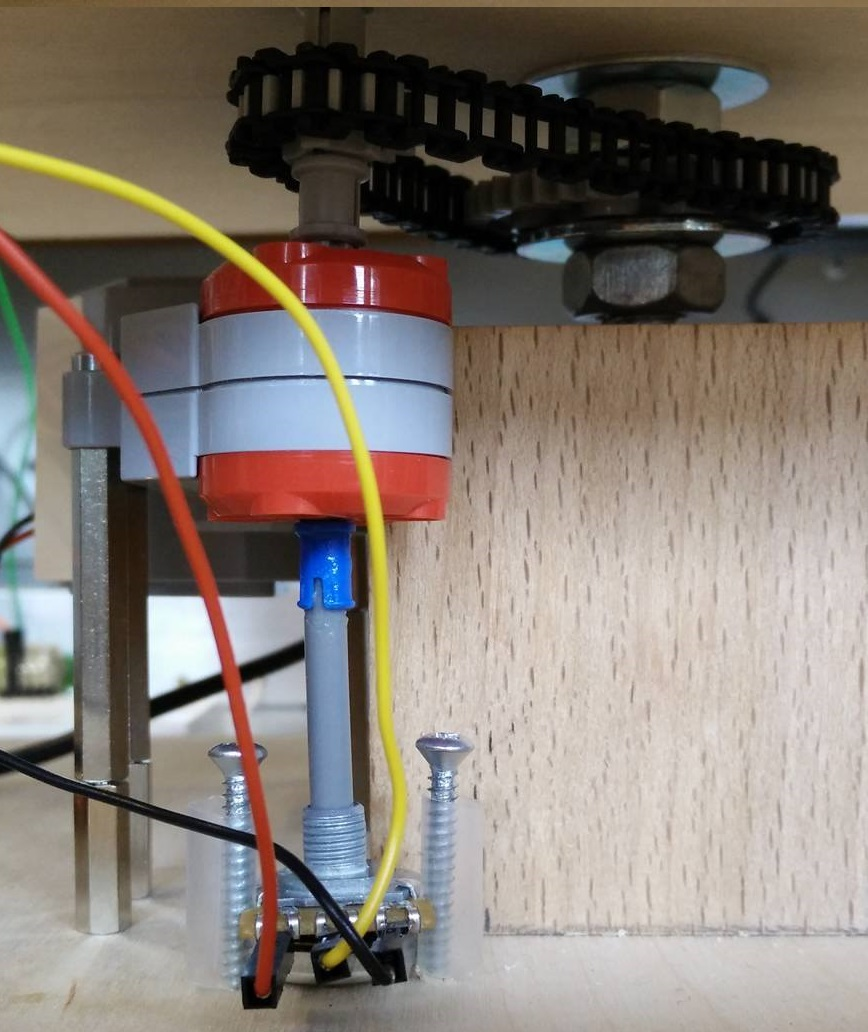
\includegraphics[scale=0.3]{Afsnit/DesignOgImplementering/images/potentiometerADC}
	\caption{Opstilling for rotationsbegrænsning}
	\label{fig:opstillingADC}
\end{figure}

\noindent \textbf{Potentiometer} \newline
\noindent Den første del af rotationsbegrænsningen er et potentiometer, som fungerer efter spændingsdelerprincippet, som vist på figur \ref{fig:potentiometer2}.

\begin{figure}[H]
	\centering
	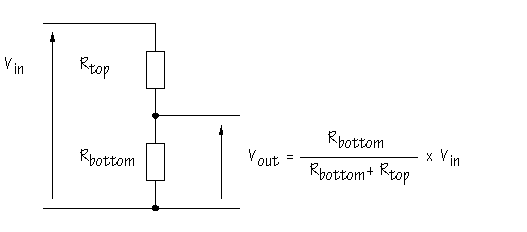
\includegraphics[scale=0.65]{DesignOgImplementering/images/potentiometer}
	\caption{Spændingsdeler formlen for potentiometeret}
	\label{fig:potentiometer2}
	
\end{figure}

\noindent Det anvendte potentiometer har en størrelse på 47\(\ K\Omega\). Denne er lineær. Det vil sige at spændingen stiger proportionalt med modstanden. I potentiometeret findes en roterende kontakt, der danner en justerbar spændingsdeler. Når skaftet på potentiometret roteres ændres modstanden i de to variable modstande, \(\ R_{1}\) og  \(\ R_{2}\). På figur \ref{fig:potentiometer2} ses en konceptuel afbildning af de variable modstande i potentiometret, hvor der ses at udgangsspændingen er spændingen over \(\ R_{1}\). \newline

\noindent \textbf{ADC} \newline
For at kunne aflæse spændingen på potentiometeret, anvendes en 12-bit AD converter af typen Sequencing Successive Approximation ADC. En sequencing SAR ADC indeholder et sample-hold kredsløb. Kredsløbet holder på et indgangssignal indtil det næste signal registres på kredsløbets indgang. Dermed har converteren tid til at bestemme outputværdien. \newline \newline
\noindent ADC'en fungerer ved at midscale indstilles til halvdelen af referencespændingen. Inputsignalet sammenlignes med midscale, hvis inputsignalet er højere end midscaleværdien sættes MSB 1 og hvis signalet er lavere bliver denne sat til 0. Herefter bliver midscale værdien rekursivt sat til havdelen af intervallet, som inputsignalet ligger indenfor, og bittene ned til LSB bliver sat. Bittene der sættes, bliver gemt i et register. Når konverteringen er gennemført, kan værdien af inputsignalet aflæses i dette register. 

\begin{figure}[H]
	\centering
	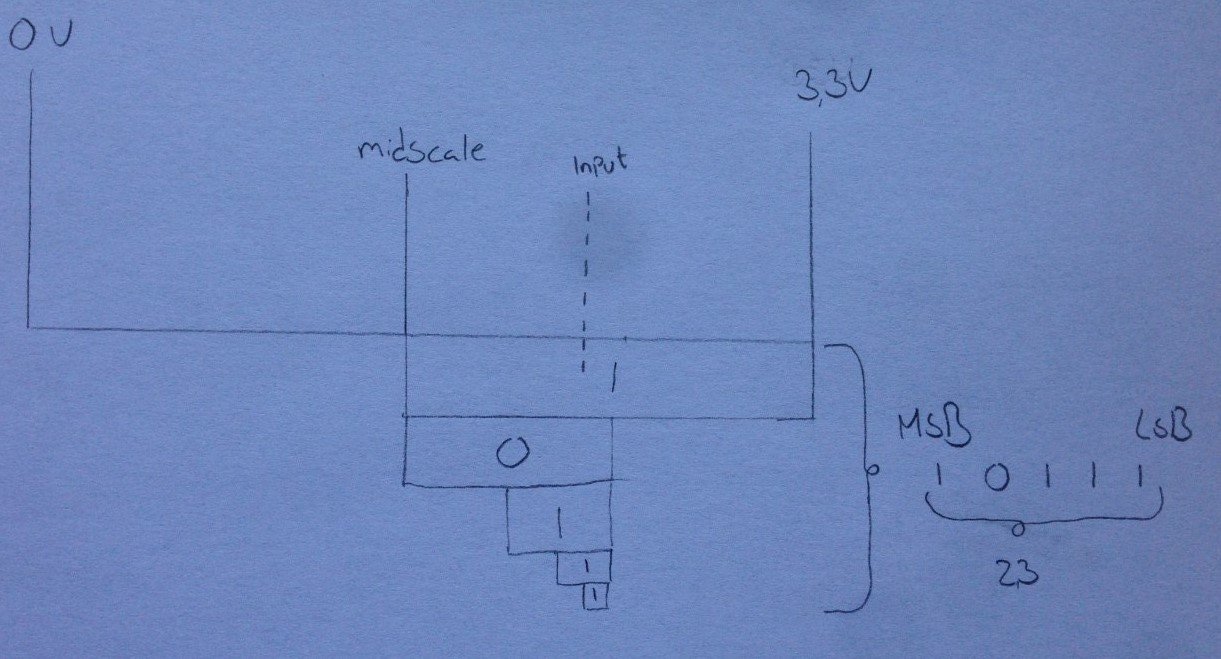
\includegraphics[width=\textwidth]{DesignOgImplementering/images/ADC}
	\caption{Illustation af AD konvertering}
	\label{fig:ADC1}
	
\end{figure}

\noindent På figur \ref{fig:ADC1} ses et eksempel over de første fem trin i en konvertering. Til dette projekt arbejdes der med en 12-bit AD converter, dermed ville denne konvertering forsætte 12 trin ned.  \newline